% !TEX root = ../main.tex
% --+ 20.14a Q2 +---------------------------------------------------------------
\begin{frame}{DIS Plots: $Q^2$}
    \label{20.14a::q2}

    \begin{figure}[t]
        \centering{
            \fbox{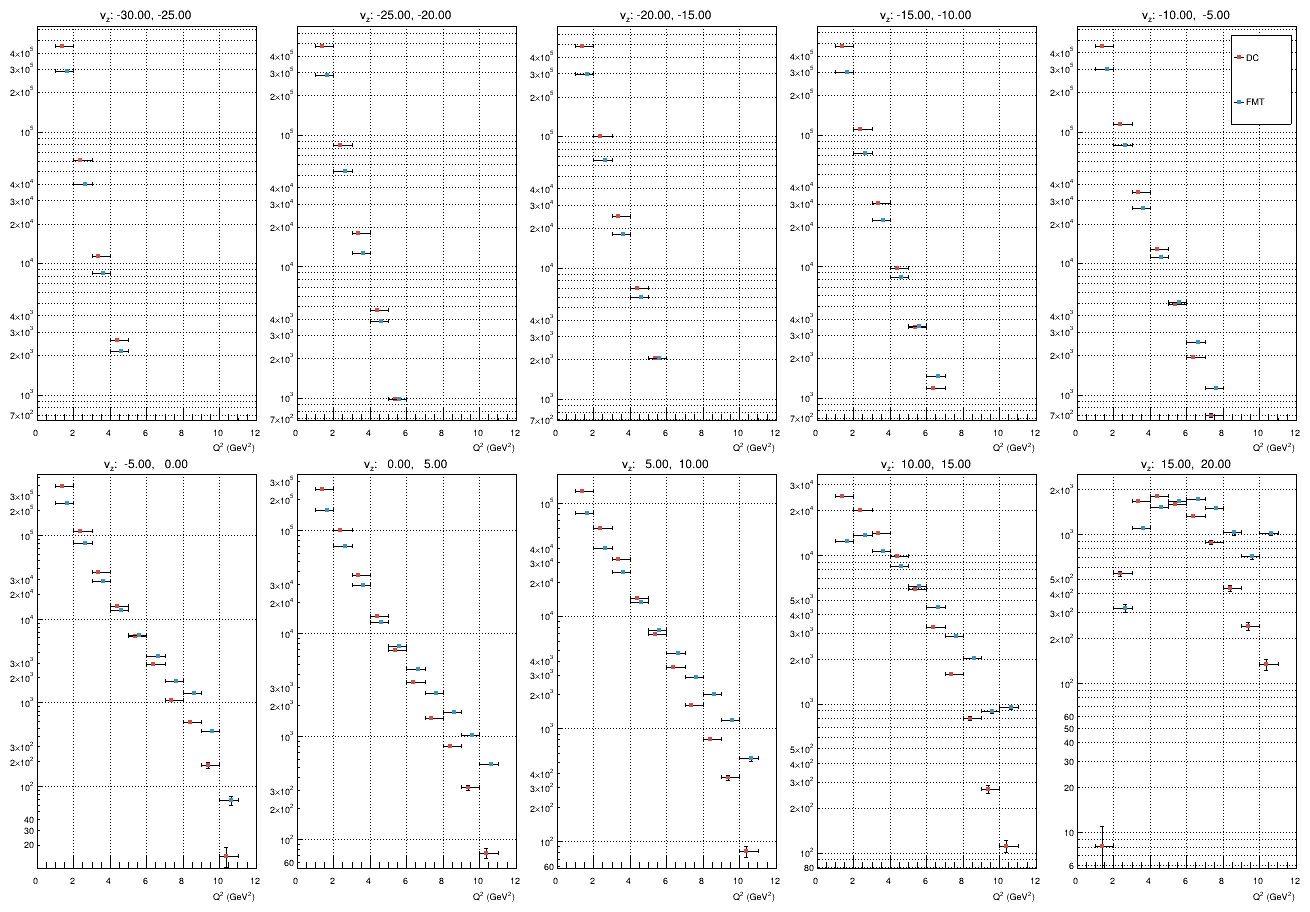
\includegraphics[width=0.72\textwidth]{14a_q2.png}}
        }
    \end{figure}

    \backref{12.12::q2}
\end{frame}

% --+ 20.14b NU +---------------------------------------------------------------
\begin{frame}{DIS Plots: $\nu$}
    \label{20.14b::nu}

    \begin{figure}[t]
        \centering{
            \fbox{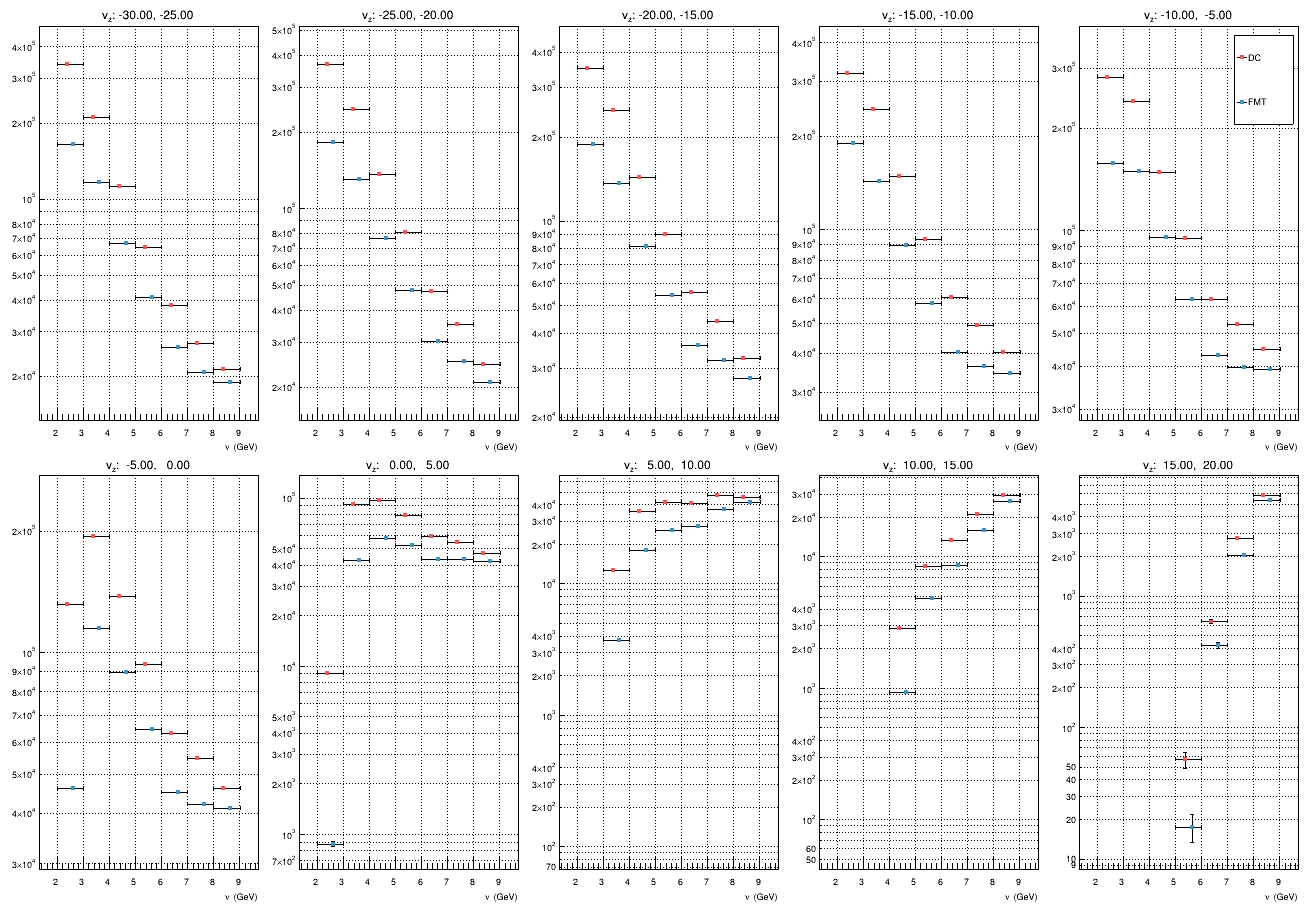
\includegraphics[width=0.72\textwidth]{14b_nu.png}}
        }
    \end{figure}

    \backref{12.13::nu}
\end{frame}

% --+ 20.14c zh pi+ +-----------------------------------------------------------
\begin{frame}{DIS Plots: $z_h$ for $\pi^+$}
    \label{20.14c::zh_pi+}

    \begin{figure}[t]
        \centering{
            \fbox{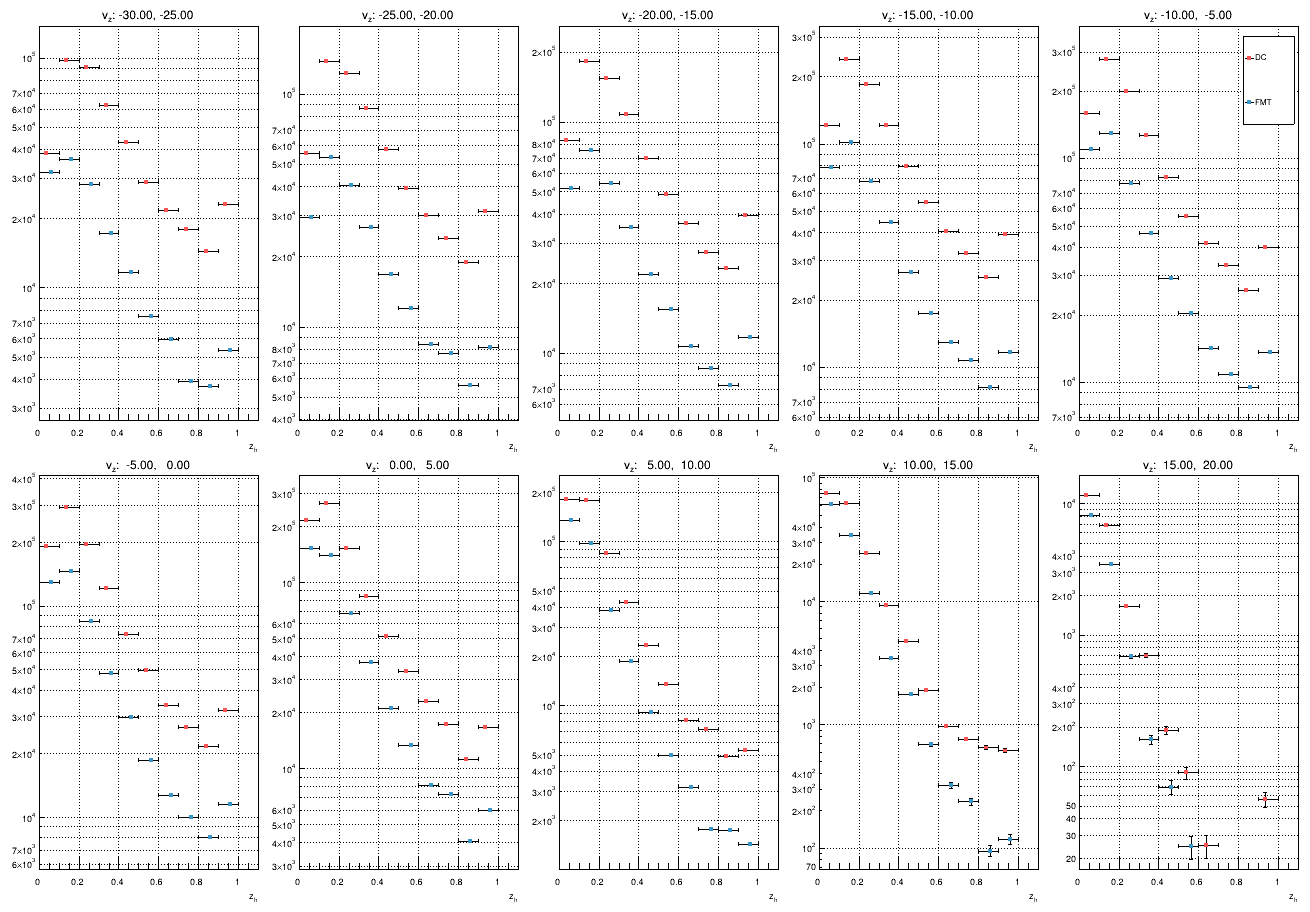
\includegraphics[width=0.72\textwidth]{14c_zh_pi+.png}}
        }
    \end{figure}

    \backref{12.14::zh}
\end{frame}

% --+ 20.14d zh pi- +-----------------------------------------------------------
\begin{frame}{DIS Plots: $z_h$ for $\pi^-$}
    \label{20.14d::zh_pi-}

    \begin{figure}[t]
        \centering{
            \fbox{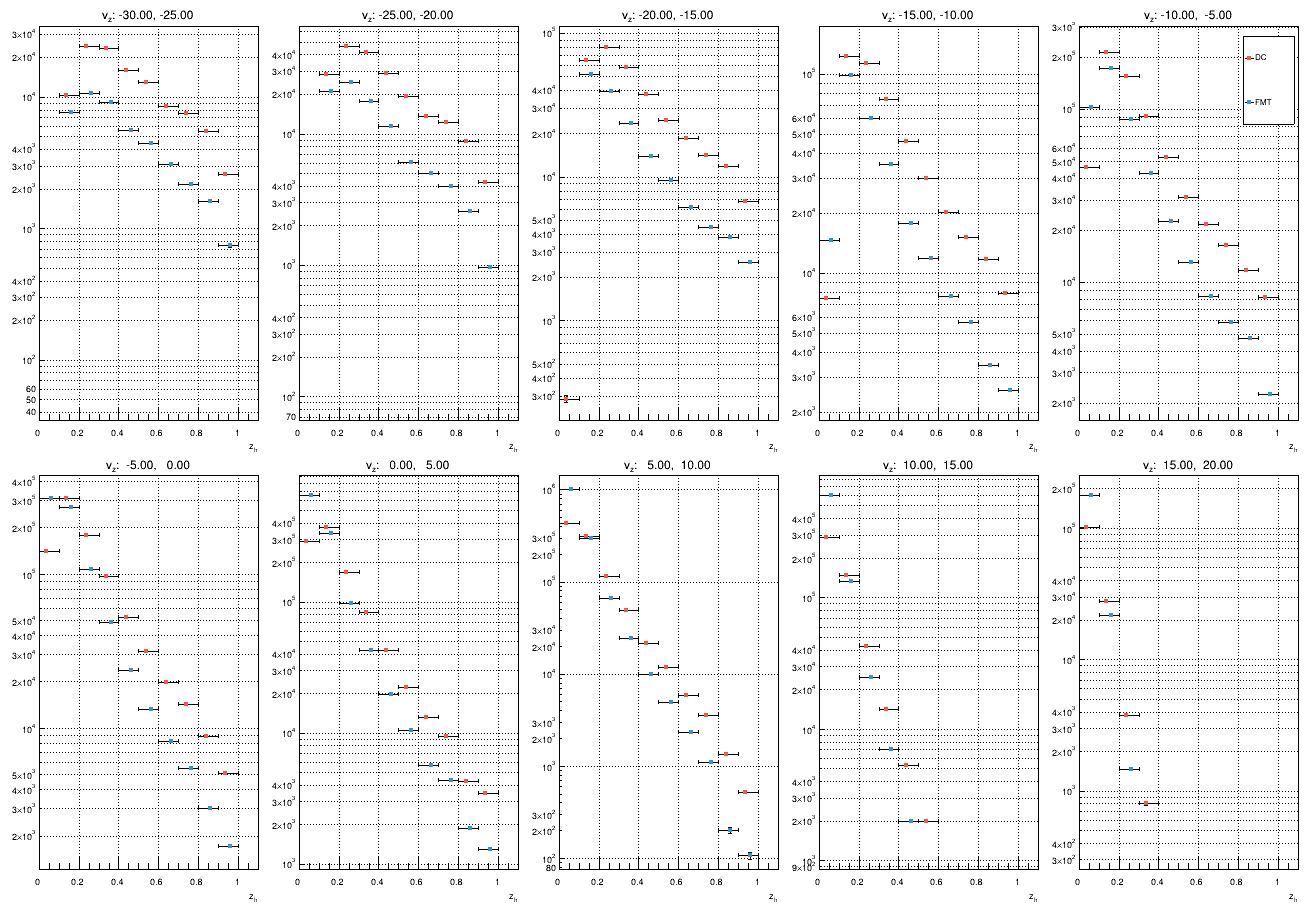
\includegraphics[width=0.72\textwidth]{14d_zh_pi-.png}}
        }
    \end{figure}

    \backref{12.14::zh}
\end{frame}

% --+ 20.14e pt2 pi+ +----------------------------------------------------------
\begin{frame}{DIS Plots: $p_T^2$ for $\pi^+$}
    \label{20.14e::pt2_pi+}

    \begin{figure}[t]
        \centering{
            \fbox{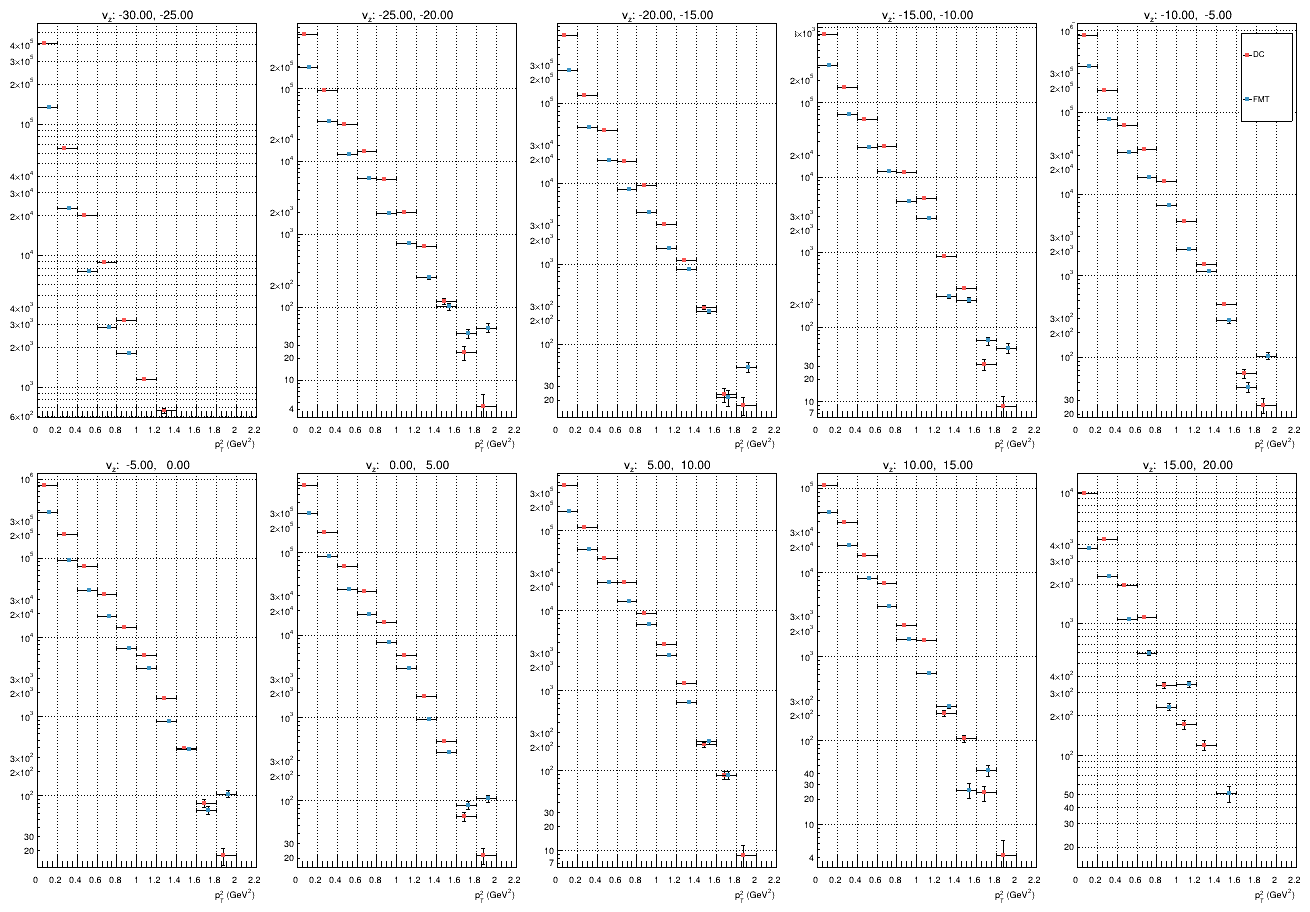
\includegraphics[width=0.72\textwidth]{14e_pt2_pi+.png}}
        }
    \end{figure}

    \backref{12.15::pt2}
\end{frame}

% --+ 20.14f pt2 pi- +----------------------------------------------------------
\begin{frame}{DIS Plots: $p_T^2$ for $\pi^-$}
    \label{20.14f::pt2_pi-}

    \begin{figure}[t]
        \centering{
            \fbox{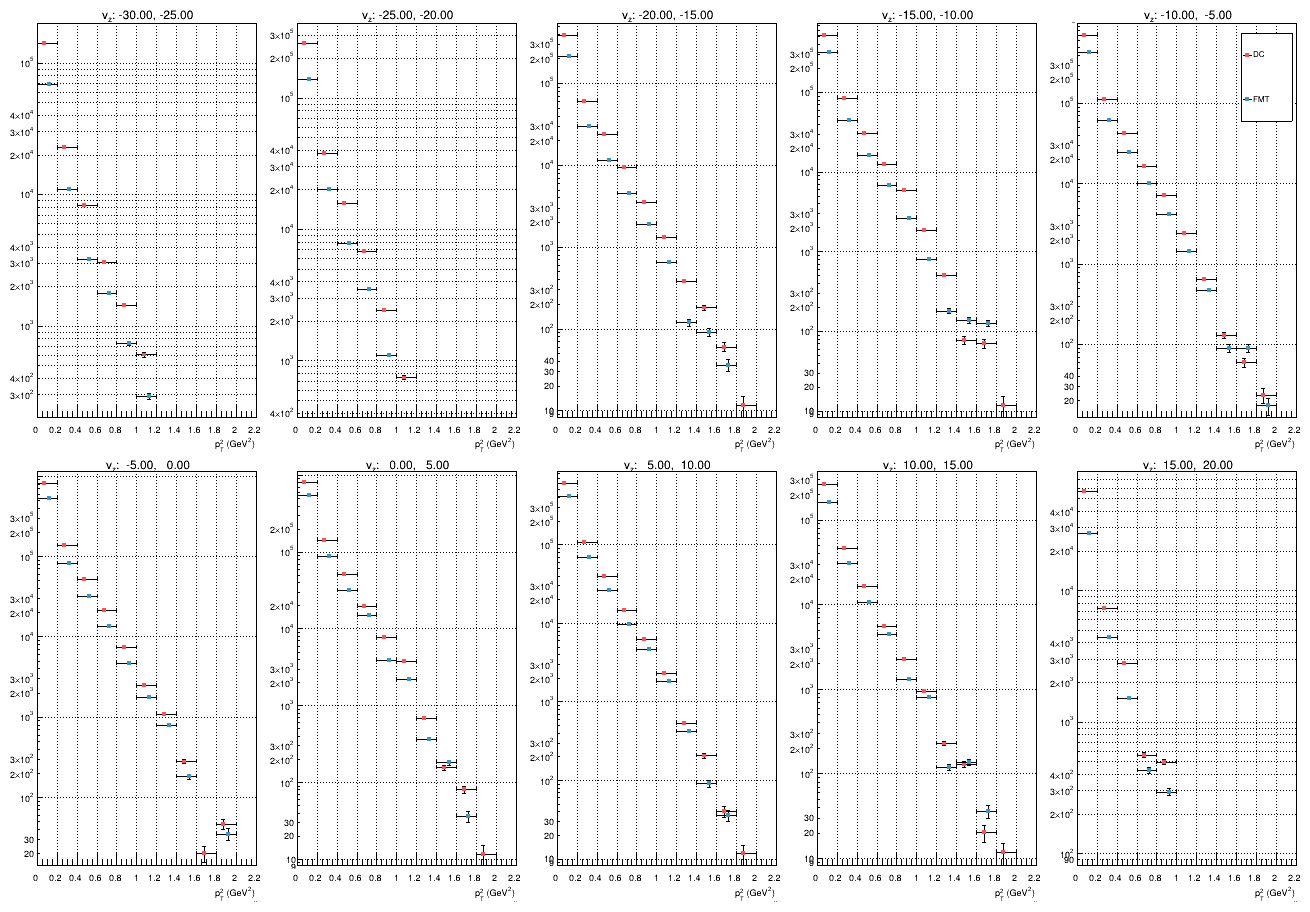
\includegraphics[width=0.72\textwidth]{14f_pt2_pi-.png}}
        }
    \end{figure}

    \backref{12.15::pt2}
\end{frame}

% --+ 20.14g phipq pi+ +--------------------------------------------------------
\begin{frame}{DIS Plots: $\phi_{PQ}$ for $\pi^+$}
    \label{20.14g::phipq_pi+}

    \begin{figure}[t]
        \centering{
            \fbox{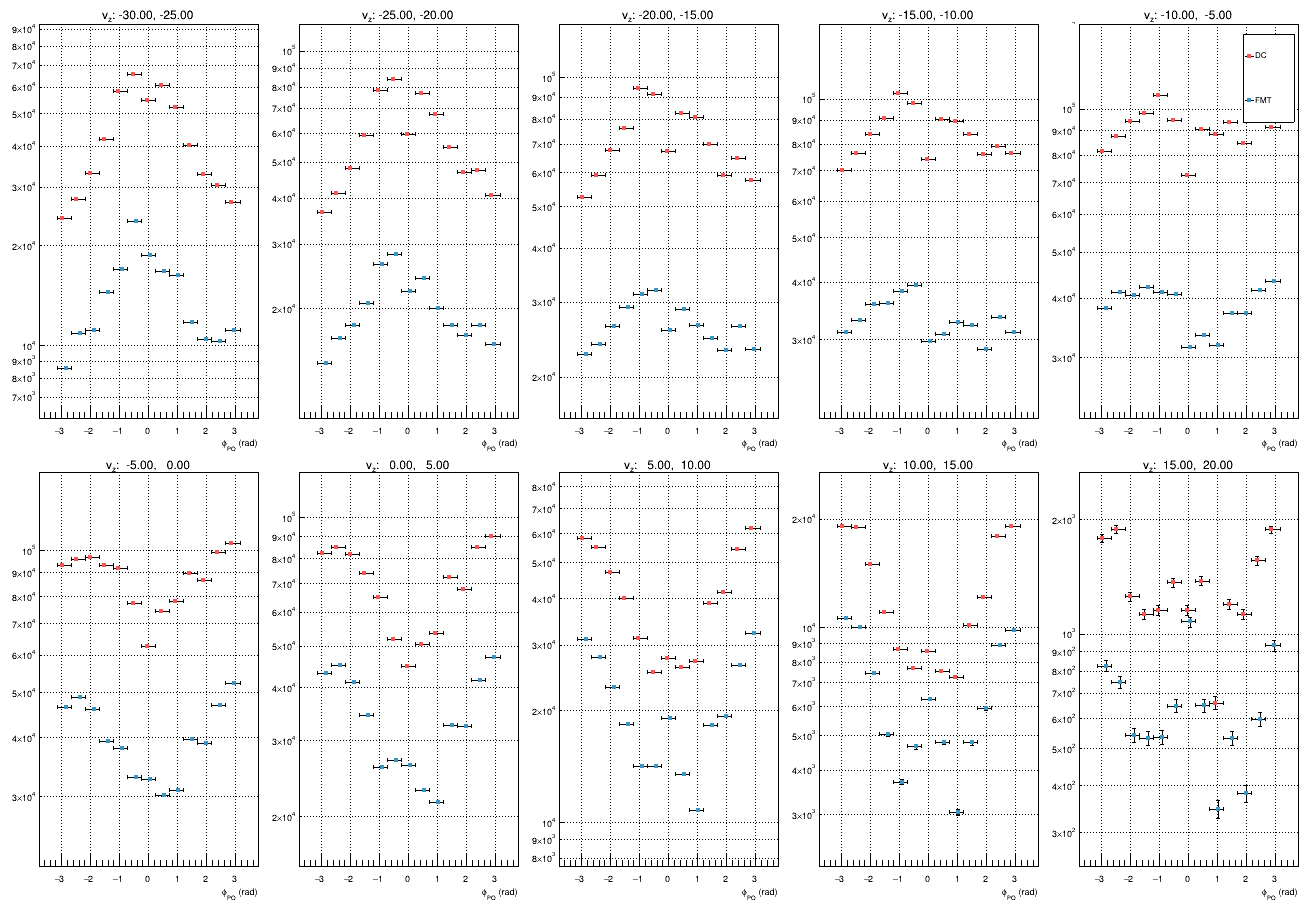
\includegraphics[width=0.72\textwidth]{14g_phipq_pi+.png}}
        }
    \end{figure}

    \backref{12.16::phipq}
\end{frame}

% --+ 20.14h phipq pi- +--------------------------------------------------------
\begin{frame}{DIS Plots: $\phi_{PQ}$ for $\pi^-$}
    \label{20.14h::phipq_pi-}

    \begin{figure}[t]
        \centering{
            \fbox{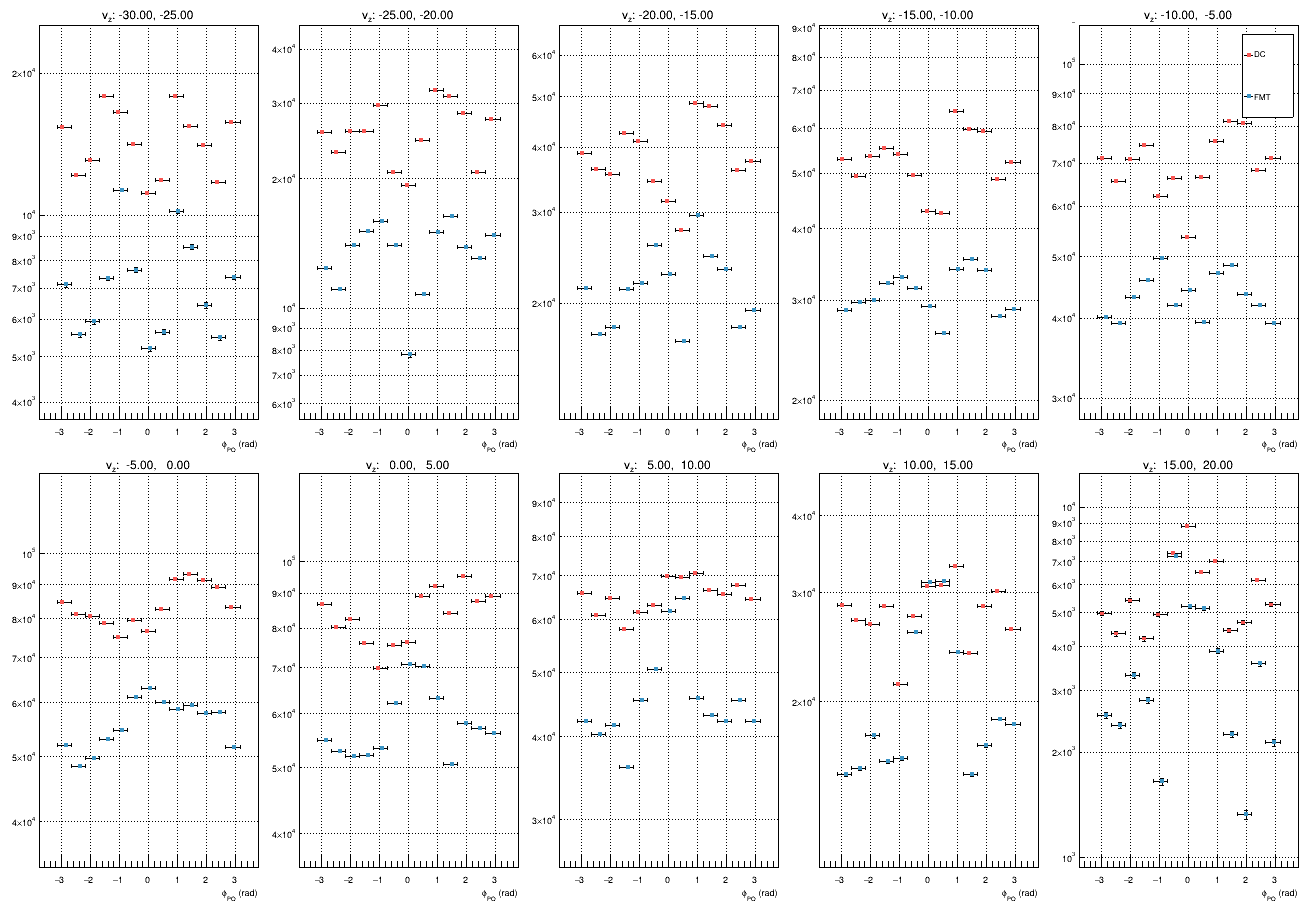
\includegraphics[width=0.72\textwidth]{14h_phipq_pi-.png}}
        }
    \end{figure}

    \backref{12.16::phipq}
\end{frame}
